% !TEX encoding = UTF-8 Unicode
%!TEX TS-program = xelatex

\documentclass[12pt]{extarticle}
% extarticle is like article but can handle 8pt, 9pt, 10pt, 11pt, 12pt, 14pt, 17pt, and 20pt text

\def \ititle {Origins of Mind}
 
\def \isubtitle {Lecture 08}
 
\def \iauthor {Stephen A. Butterfill}
\def \iemail{s.butterfill@warwick.ac.uk}
\date{}

%for strikethrough
\usepackage[normalem]{ulem}

\usepackage{pdfpages}


\input{$HOME/Documents/submissions/preamble_steve_handout}

%logic symbol \leftmodels
\usepackage{MnSymbol}

%\bibpunct{}{}{,}{s}{}{,}  %use superscript TICS style bib
%remove hanging indent for TICS style bib
%TODO doesnt work
\setlength{\bibhang}{0em}
%\setlength{\bibsep}{0.5em}


%itemize bullet should be dash
\renewcommand{\labelitemi}{$-$}

\begin{document}

%\raggedcolumns

\begin{multicols*}{3}

\setlength\footnotesep{1em}


\bibliographystyle{newapa} %apalike

%\maketitle
%\tableofcontents




%--------------- 
%--- start paste
\def \ititle {Logic (PH133)}
 
\def \isubtitle {Lecture 8}
 
\begin{center}
 
{\Large
 
\textbf{\ititle}: \isubtitle
 
}
 
 
 
\iemail %
 
\end{center}
 
Readings refer to sections of the course textbook, \emph{Language, Proof and Logic}.
 
 
 
\section{There Is a Store for Everything}
 
\emph{Reading:} §11.2, §11.3
 
There is a store for everything:
 
\hspace{3mm}	∃y∀x StoreFor(y,x)
 
\hspace{3mm} ∀y∃x StoreFor(x,y)
 
Other sentences to translate:
 
\hspace{3mm} Wikipedia has an article about everything
 
\hspace{3mm} Everyone hurts someone they love
 
\hspace{3mm} Someone hurts everyone she loves
 
 
 
\section{Variables}
 
Names : a, b, c, …
 
Variables : x, y, z, w, …
 
Variables are for saying several things about one thing even without specifying which thing it is
 
NB: `Some x is a horse and x is dead' ain't English.
 
 \columnbreak
 
\section{Loving and Being Loved}
 
\emph{Reading:} §11.2, §11.3
 
\begin{center}
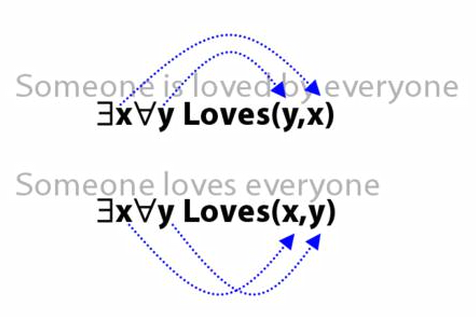
\includegraphics[scale=0.3]{img/unit_755_loved.png}
\end{center}
 
 
\section{There Does Not Exist}
 
Something is not dead:
 
\hspace{3mm} ∃x ¬Dead(x)
 
Nothing is dead:
 
\hspace{3mm} ¬∃x Dead(x)
 
Everything is not broken:
 
\hspace{3mm} ∀x ¬Broken(x)
 
Not everything is broken:
 
\hspace{3mm} ¬∀x Broken(x)
 
\begin{center}
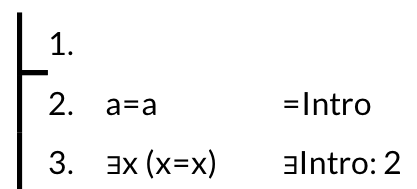
\includegraphics[scale=0.3]{img/unit_605_prf1.png}
\end{center}
\begin{center}
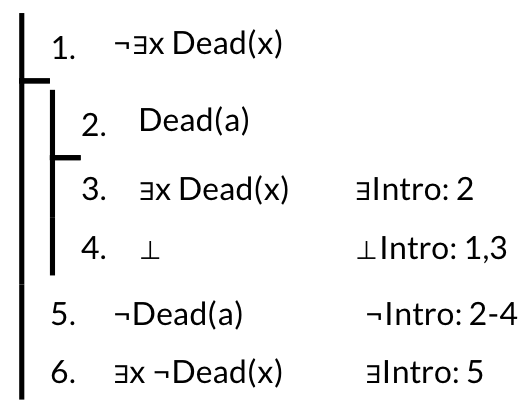
\includegraphics[scale=0.3]{img/unit_605_prf2.png}
\end{center}
\begin{center}
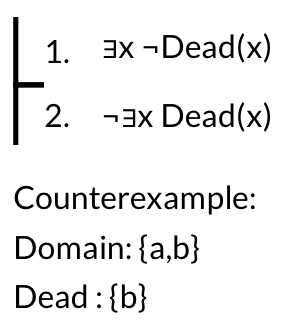
\includegraphics[scale=0.3]{img/unit_605_counterexample.png}
\end{center}
 
 
\section{Quantifier Equivalences: \\ ¬∀x Created(x) $\leftmodels\models$ ∃x ¬Created(x)}
 
\emph{Reading:} §10.1, §10.3, §10.4
 
 
 
\section{Proof Example: \\ ∃x Dead(x) $\vdash$ ¬∀x¬ Dead(x).}
 
\begin{center}
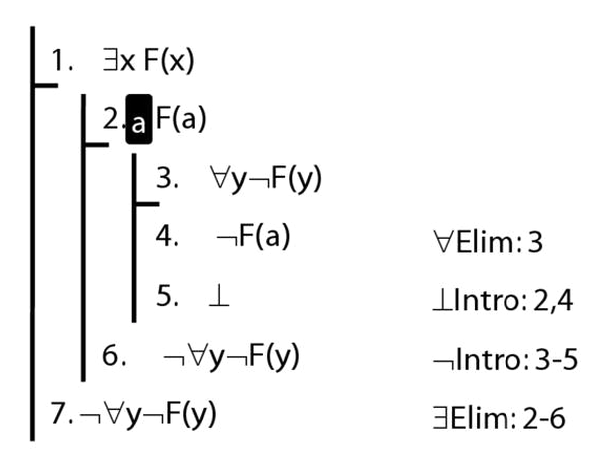
\includegraphics[scale=0.3]{img/unit_825_proof.png}
\end{center}
 
 
\section{Proof Example: \\ ¬∀x Dead(x) $\vdash$ ∃x¬ Dead(x).}
 
\begin{center}
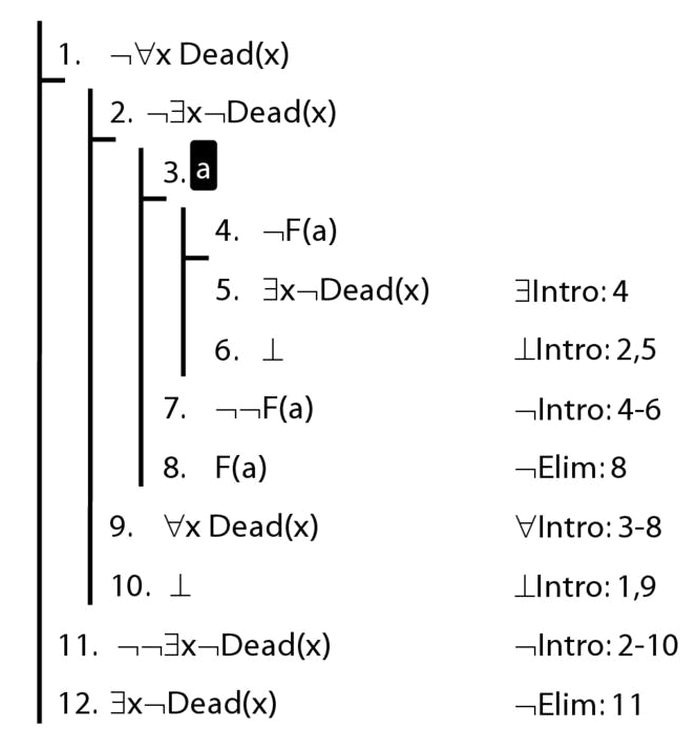
\includegraphics[scale=0.3]{img/unit_826_proof.png}
\end{center}
 
 
\section{Somebody Is Not Dead}
 
Some person is dead.
 
\hspace{5mm} ∃x(Person(x) ∧ Dead(x))
 
Some person is not dead.
 
\hspace{5mm} ∃x(Person(x) ∧ ¬Dead(x))
 
No person is dead.
 
\hspace{5mm} ¬∃x(Person(x) ∧ Dead(x))
 
Every person is dead.
 
\hspace{5mm} ∀x(Person(x) → Dead(x))
 
Every person is not dead.
 
\hspace{5mm} ∀x(Person(x) → ¬Dead(x))
 
Not every person is dead.
 
\hspace{5mm} ¬∀x(Person(x) → Dead(x))
 
 
 
\section{The End Is Near}
 
\emph{Reading:} §14.3
 
‘The’ can be a quantifier, e.g. ‘the square is broken’. How to formalise it?
 
The square is broken
\\ 
$\leftmodels\models$ There is exactly one square and it is broken
 
Recall that we can translate `There is exactly one square' as:
 
\hspace{5mm} ∃x ( Square(x) ∧ ∀y ( Square(y) → x=y ) )
 
So `There is exactly one square and it's broken':
 
∃x ( Sqr(x) ∧ ∀y ( Sqr(y) → x=y ) ∧ Broken(x) )
 
\vfill

%--- end paste
%--------------- 
 


\end{multicols*}

\end{document}